\documentclass[
  bibliography=totoc,     % Literatur im Inhaltsverzeichnis
  captions=tableheading,  % Tabellenüberschriften
  titlepage=firstiscover, % Titelseite ist Deckblatt
]{scrartcl}

% Paket float verbessern
\usepackage{scrhack}

% Warnung, falls nochmal kompiliert werden muss
\usepackage[aux]{rerunfilecheck}

% unverzichtbare Mathe-Befehle
\usepackage{amsmath}
% viele Mathe-Symbole
\usepackage{amssymb}
% Erweiterungen für amsmath
\usepackage{mathtools}

% Fonteinstellungen
\usepackage{fontspec}
% Latin Modern Fonts werden automatisch geladen
% Alternativ:
%\setromanfont{Libertinus Serif}
%\setsansfont{Libertinus Sans}
%\setmonofont{Libertinus Mono}
\recalctypearea % Wenn man andere Schriftarten gesetzt hat,
% sollte man das Seiten-Layout neu berechnen lassen

% deutsche Spracheinstellungen
\usepackage{polyglossia}
\setmainlanguage{german}


\usepackage[
  math-style=ISO,    % ┐
  bold-style=ISO,    % │
  sans-style=italic, % │ ISO-Standard folgen
  nabla=upright,     % │
  partial=upright,   % ┘
  warnings-off={           % ┐
    mathtools-colon,       % │ unnötige Warnungen ausschalten
    mathtools-overbracket, % │
},                       % ┘
]{unicode-math}

% traditionelle Fonts für Mathematik
\setmathfont{Latin Modern Math}
% Alternativ:
%\setmathfont{Libertinus Math}

\setmathfont{XITS Math}[range={scr, bfscr}]
\setmathfont{XITS Math}[range={cal, bfcal}, StylisticSet=1]

% Zahlen und Einheiten
\usepackage[
locale=DE,                   % deutsche Einstellungen
separate-uncertainty=true,   % immer Fehler mit \pm
per-mode=symbol-or-fraction, % / in inline math, fraction in display math
]{siunitx}

% chemische Formeln
\usepackage[
version=4,
math-greek=default, % ┐ mit unicode-math zusammenarbeiten
text-greek=default, % ┘
]{mhchem}

% richtige Anführungszeichen
\usepackage[autostyle]{csquotes}

% schöne Brüche im Text
\usepackage{xfrac}

% Standardplatzierung für Floats einstellen
\usepackage{float}
\floatplacement{figure}{htbp}
\floatplacement{table}{htbp}

% Floats innerhalb einer Section halten
\usepackage[
section, % Floats innerhalb der Section halten
below,   % unterhalb der Section aber auf der selben Seite ist ok
]{placeins}

% Seite drehen für breite Tabellen: landscape Umgebung
\usepackage{pdflscape}

% Captions schöner machen.
\usepackage[
  labelfont=bf,        % Tabelle x: Abbildung y: ist jetzt fett
  font=small,          % Schrift etwas kleiner als Dokument
  width=0.9\textwidth, % maximale Breite einer Caption schmaler
]{caption}
% subfigure, subtable, subref
\usepackage{subcaption}

% Grafiken können eingebunden werden
\usepackage{graphicx}
% größere Variation von Dateinamen möglich
\usepackage{grffile}

% schöne Tabellen
\usepackage{booktabs}

% Verbesserungen am Schriftbild
\usepackage{microtype}

% Literaturverzeichnis
\usepackage[style=alphabetic,]{biblatex}
% Quellendatenbank
\addbibresource{lit.bib}
\addbibresource{programme.bib}

% Hyperlinks im Dokument
\usepackage[
  unicode,        % Unicode in PDF-Attributen erlauben
  pdfusetitle,    % Titel, Autoren und Datum als PDF-Attribute
  pdfcreator={},  % ┐ PDF-Attribute säubern
  pdfproducer={}, % ┘
]{hyperref}
% erweiterte Bookmarks im PDF
\usepackage{bookmark}

% Trennung von Wörtern mit Strichen
\usepackage[shortcuts]{extdash}

\title{V01: Lebensdauer von Myonen}
\author{
  Simon Schulte
  \texorpdfstring{
    \\
    \href{mailto:simon.schulte@udo.edu}{simon.schulte@udo.edu}
  }{}
  \texorpdfstring{\and}{, }
  Tim Sedlaczek
  \texorpdfstring{
    \\
    \href{mailto:tim.sedlaczek@udo.edu}{tim.sedlaczek@udo.edu}
  }{}
}
\publishers{TU Dortmund – Fakultät Physik}

\date{Durchführung: 23.04.2018\\
      Erstabgabe: 03.05.2018\\
      Korrekturabgabe: 02.07.2018}


\begin{document}

\maketitle
\thispagestyle{empty}
\setcounter{page}{1}
\pagenumbering{arabic}
\section{Theorie}
\label{sec:theorie}
  Ziel des Versuchs ist die Bestimmung der Lebensdauer von Myonen. Myonen
  entstehen unter anderem in Luftschauern in der Hochatmosphäre durch
  Pionzerfälle. Diese Pionen widerum entstehen zum Beispiel aus kosmischen
  Protonen aus u.A. Aktiven Galaktischen Kernen. Solche Protonen haben eine sehr
  hohe kinetische Energie. Das führt dazu, dass die entstehenden Myonen
  relativistische Geschwindigkeiten aufweisen und sie somit trotz ihrer kurzen
  Lebensdauer auf der Erdoberfläche registrierbar sind.
    \subsection{Standardmodell}
    \label{sec:standardmodell}
  Das Standardmodell unterscheidet zwischen zwei Arten von Elementarteilchen.
  Diese zwei Arten sind zum ersten (Eich)Bosonen und außerdem Fermionen.
  Während Bosonen als Austauschteilchen der fundamentalen Wechselwirkungen fungieren,
  stellen Fermionen die kleinsten aktuell bekannten Bausteine der Materie dar.
  Die Fermionen werden dabei in Quarks und Leptonen unterteilt. Quarks bilden
  dabei die fundamentalen Bausteine der Hadronen. Dazu gehören unter Anderem
  auch Protonen und Pionen, die für diesen Versuch von Relevanz sind.
  Leptonen und Quarks sind in drei Generationen aufgeteilt. Die
  Leptongenerationen sind:
  \begin{itemize}
    \item[I] Elektron ($\symup{e}^-$) und Elektron-Neutrino ($\symup\nu_{\symup{e}}$)
    \item[II] Myon ($\symup\mu^-$) und Myon-Neutrino ($\symup\nu_{\symup\mu}$)
    \item[III] Tauon ($\symup\tau^-$) und Tauon-Neutrino ($\symup\nu_{\symup\tau}$).
  \end{itemize}
  Dabei haben die Neutrinos eine im Standardmodell verschwindend geringe Masse.\\
  All diese Teilchen haben außerdem auch ein Antiteilchen. Das Antiteilchen
  eines geladenen Fermions hat die gleichen Eigenschaften, wie das Fermion
  selbst, außer, dass das Vorzeichen der Ladung sich ändert.
  Ein Antineutrino kennzeichnet sich durch eine Überstreichung. Sie sind
  wichtig, wenn Antifermionen an einem Zerfall beteiligt sind, um in dem
  jeweiligen Zerfall die Leptonzahlerhaltung zu gewährleisten.
  Die Lebensdauern von Myonen und Tauonen sind verschwindend gering und das
  Elektron ist das einzige stabile geladene Lepton. Dementsprechend zerfallen
  die Myonen und Tauonen bevorzugt in Elektronen. Wie bereits am Anfang erwähnt
  entstehen die meisten Myonen, die uns auf der Erdoberfläche erreichen bei
  Pionzerfällen in der Erdatmosphäre:
  \begin{equation*}
    \pi^+ \to \mu^+ + \nu_{\mu} \qquad \text{ und } \qquad \pi^- \to \mu^- + \bar{\nu}_{\mu} .
    \label{pionzerfälle}
  \end{equation*}
  \subsection{Myonen in Szintillationsdetektoren}
  Die Myonen werden in diesem Versuch mit einem organischen Szintillationsdetektor nachgewiesen.
  Myonen deponieren bei ihrem Durchgang durch den Szintillator einen Teil ihrer
  kinetischen Energie im Szintillatormaterial.
  Das führt zu Anregungszuständen der Moleküle, bei deren Rückkehr in
  den Grundzustand Photonen frei werden. Die Photonen werden durch einen
  Sekundärelektronenvervielfacher (SEV) nachgewiesen. Ein SEV ist aufgebaut aus
  einer Photokathode, Dynoden zur Sekundärelektronenproduktion sowie
  einer Anode.\\
  Nun gibt es drei verschiedene Möglichkeiten, wie sich ein Myon verhält, dass
  auf den Szintillationsdetektor trifft.
    Die erste Möglichkeit ist, dass das Myon bereits so viel Energie in der Atmosphäre
    verloren hat, dass dieses dann im Detektor zerfällt. Zur Bestimmung der
    Lebensdauer wird dieses Verhalten beobachtet. Myonen, die im Detektor
    zerfallen, zerfallen zu nahezu $\SI{100}{\percent}$ in ein Elektron und die entsprechenden Neutrinos:
    \begin{align*}
      \mu^+ &\to e^+ + \nu_{e} + \bar{\nu}_{\mu},\\
      \mu^- &\to e^- + \bar{\nu}_{e} +  \nu_{\mu}.
    \end{align*}
    Da die Masse des Myons etwa 207 mal größer ist, als die des Elektrons folgt,
    dass so entstehende Elektronen sehr viel kinetische Energie haben. Diese
    reicht aus, um das Szintillatormaterial anzuregen. Dabei entstehen Photonen,
    die als Stoppsignal fungieren. Aus der zeitlichen Differenz von Eintritt des Myons im
    Szintillator und dem Zerfall des Myons lässt sich dann, mit einigen Methoden
    der statistischen Datenanalyse die Lebensdauer der Myonen bestimmen.\\
    Die zweite Möglichkeit ist, dass das Myon den Detektor durchquert ohne zu
    zerfallen. Dann wird trivialerweise immernoch das erste Signal detektiert,
    aber das zweite nicht. Das führt zu einem Untergrundrauschen. Diesem
    Untergrundrauschen wird mit dem verwendeten Versuchsaufbau entgegengewirkt.\\
    Die letzte Möglichkeit ist, dass negative Myonen durch die Szintillatoratome
    eingefangen werden. Wie bei der zweiten Möglichkeit wird dann ebenfalls
    das erste Signal detektiert und zusätzlich kann durch den Zerfall des Myons
    ein weiteres Signal detektiert werden.
  \subsection{Teilchenzerfälle}
  \label{sec:teilchenzerfälle}
  Die Teilchenzerfälle sind statistische Prozesse.
  Die Wahrscheinlichkeit $\symup{d}W$,
  dass ein Zerfall im Zeitraum $\symup{d}t$ eintritt, ergibt sich zu:
  \begin{equation*}
    \symup{d}W = \lambda\symup{d}t,
  \end{equation*}
  $\lambda$ stellt hier eine charakteristische Zerfallskonstante dar.
  Es fällt auf, dass die Wahrscheinlichkeit für einen Zerfall unabhängig
  vom individuellen Alter des Teilchens ist. Die Lebensdauer eines Teilchens ist
  nur eine Angabe für den wahrscheinlichsten Zeitpunkt des Zerfalls von dem
  jeweiligen Teilchen. Außerdem sind die Zerfälle einer Vielzahl von Teilchen
  unabhängig voneinander. Für die Zahl der Teilchen $\symup{d}N$, die im
  Zeitraum $\symup{d}t$ zerfallen sind folgt:
  \begin{equation*}
    \symup{d}N = -N\symup{d}W = - \lambda N \symup{d}t.
  \end{equation*}
  Durch Integration lässt sich auf das exponentielle Zerfallsgesetz schließen:
  \begin{equation}
    \frac{N(t)}{N_0} = \exp{(-\lambda t)}.
    \label{eq:expozerfall}
  \end{equation}
  Dabei bezeichnet $t$ die Zeit und $N_0$ die Anzahl vorhandener
  Teilchen zum Zeitpunkt $t=0$. Die Verteilungsfunktion in einem Intervall
  $[t, \symup{d}t]$ ergibt sich zu:
  \begin{equation*}
    \symup{d}N \left( t \right) = N_0 \cdot \lambda \cdot \symup{exp} \left( - \lambda t \right) \symup{d}t \; .
  \end{equation*}
  Wenn der erste Moment dieser Verteilung bestimmt wird, ergibt sich ein
  Erwartungswert für die Lebensdauer:
  \begin{equation}
    <t> = \tau = \int_0^\infty \lambda t \exp{(-\lambda t)} \symup{d}t =
    \left| \lambda \left( -\frac{t}{\lambda} - \frac{1}{\lambda^2} \right)\exp{(-\lambda t)}
    \right|_0^\infty = \frac{1}{\lambda}.
    \label{eq:tau}
  \end{equation}
  \subsection{Statistische Probleme}
  Wäre es möglich, $N \to \infty$ Teilchen zu betrachten, würden die Messwerte gegen die
  im Kapitel $\ref{sec:teilchenzerfälle}$
  bestimmte Verteilungsfunktion \eqref{eq:expozerfall} konvergieren. Gemessen
  wird allerdings nur für etwa 42 Stunden. Dadurch ergibt sich das
  arithmetische Mittel als gute Näherung, um den Erwartungswert der Stichprobe
  zu bestimmen, da bei diesem keine Messwerte ausgeschlossen werden. Dies
  ist hier aber nicht sinnvoll, da einige der Daten durch Untergrund zu Stande
  kommen. Durch eine nichtlineare Ausgleichsrechnung kann diese Näherung
  allerdings noch präzisiert werden. Dafür wird die Methode der kleinsten
  Fehlerquadrate genutzt. Die Lebensdauer wird durch
  Regression durch die Messwerte mit der Verteilungsfunktion abgeschätzt.
\section{Durchführung}
  \subsection{Versuchsaufbau}
  \label{sec:Aufbau}
  	Abbildung \ref{fig:aufbau} zeigt die im Versuch verwendete Schaltung.
  	Der hier verwendete organische Szintillator befindet sich dabei in einem
    Edelstahlzylinder, an dessen Enden jeweils ein SEV optisch angekoppelt ist.
    Dabei ist dieser Szintillator ein organischer Szintillator, weil das
    Szintillatormedium in Toluol gelöst ist. Organische Szintillatoren besitzen
    eine kürzere Abklingdauer und eignen sich daher für diesen Versuch. Anorganische
    Szintillatoren haben hingegen eine bessere Energieauflösung.\\
  	Ziel ist es, die Zeit zwischen dem ersten Lichtimpuls, der durch das
    Eindringen des Teilchens in den Detektor erzeugt wird und dem zweiten
    Lichtimpuls, der durch den Zerfall des Teilchens im Detektor erzeugt wird,
    zu bestimmen. Dies wird mit einem Zeit-Amplituden-Konverter (TAC) realisiert.
    Der TAC gibt einen Spannungsimpuls ab, dessen Höhe proportional zum zeitlichen Abstand der
  	beiden Signale ist. Zum Bestimmen dieser Zeitabstände wird eine Stopp-Uhr genutzt.
    Der erste Impuls startet das Zählwerk, der zweite Impuls stoppt es.
    Der am TAC entstehende Impuls wird anschließend in einem Vielkanalanalysator
  	entsprechend seiner Höhe in einen Kanal eingeordnet und gespeichert.
  	Die Daten werden über einen Rechner mit dem Programm \textsc{Maestro} ausgelesen.
    \newpage
  	\begin{figure}[H]
    	\centering
    	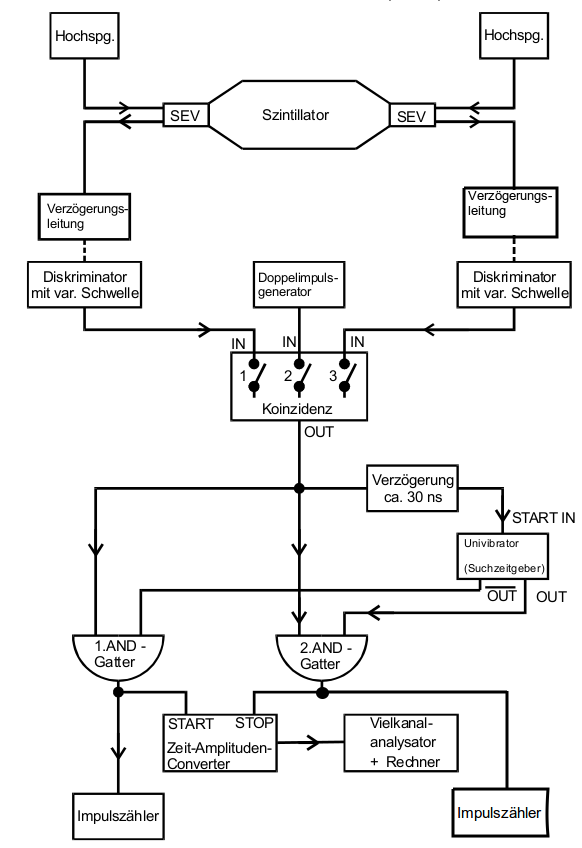
\includegraphics[width=0.7\textwidth]{Bilder/AufbauB.png}
    	\caption{Ein Blockschaltbild des Versuchsaufbaus, nach [Phy18] mit kleinen Änderungen.}
    	\label{fig:aufbau}
  	\end{figure}
  \subsubsection{Filtern von nicht-zerfallenden Myonen.}
  Die im vorherigen Kapitel beschriebene Messmethode ist nicht geeignet, um die in Kapitel
  \ref{sec:teilchenzerfälle} beschriebenen Fälle auszuschließen, in denen das Myon
  nicht zerfällt, also nur der Eintrittslichtimpuls im Szintillator entsteht.
  Neben dem bereits im vorherigen Kapitel erwähntem Untergrund, welches durch zu
  schnell einfallende Myonen entsteht, gibt es außerdem noch andere Untergrundquellen.
  Dazu gehören spontane, thermische Elektronenemissionen
  der SEVs. Diese führen zu Spannungssignalen, obwohl kein Myon eingefallen ist.
  Die entstehenden Signale sind jedoch meistens kleiner als die, die von Myonen verursacht werden.
  Zur Unterdrückung dieser Signale werden zum ersten Diskriminatoren eingesetzt, die
  den beiden SEVs nachgeschaltet sind. Die Diskriminatoren geben nur dann ein Signal
  ab, wenn das einlaufende Signal eine gewisse Schwelle überschreitet. Die
  Diskriminatoren leisten dabei weiterhin eine Umwandlung der einfallenden Pulse
  in ein H-Signal der NIM-Logik.
  Zum zweiten wird eine Koinzidenzschaltung genutzt. Gefiltert wird hier, indem nur
  wenn von beiden SEVs innerhalb einer Zeit $\symup\Delta t_K$
  ein Signal an den Eingängen der Koinzidenz ankommt, ein Signal weitergegeben wird.
  Spontane Emissionen betreffen in der Regel nur einen SEV. Die Wahrscheinlichkeit,
  dass es nun an beiden SEVs gleichzeitig zu einer spontanen Emission kommt ist relativ gering.
  Die Zeit $\symup\Delta t_K$
  ist durch Variation der Diskriminatorlänge so gewählt, dass Sie sowohl den Lichtweg zwischen den beiden SEVs,
  der bei ca. \SI{4}{\nano\second} für den Fall, dass ein Signal unmittelbar an einem SEV
  entsteht, liegt, als auch Unterschiede in den Kabellängen der beiden Leitungen der
  SEVs zur Koinzidenz berücksichtigt. Letzteres wird durch die unterschiedlichen
  elektrischen Eigenschaften der SEVs aufeinander abgeglichen. Außerdem wird durch das
  Einbauen einer monostabilen Kippstufe mit einer Suchzeit $T_s$, auch Univibrator genannt, das Untergrundrauschen gefiltert. Die
  monostabile Kippstufe wird dabei durch den vom SEV über eine Koinzidenzschaltung einlaufenden
  Impuls nach einer Verzögerung angestoßen und in einen instabilen Zustand gehoben.
  Im instabilen Zustand wird das an den beiden Ausgängen des Univibrators anliegende Signal so
  getauscht, dass ein H-Signal auf das 2. AND-Gatter und ein L-Signal auf das 1. AND-Gatter
  gegeben wird. Nachdem die Suchzeit abgelaufen ist, werden die Signale wieder zurückgetauscht.\\
  Läuft nun der Einfallimpuls in die Schaltung, so liegen am 1. AND-Gatter zwei
  \SI{30}{\nano\second} an. Die Verzögerung vor dem Univibrator sorgt dafür, dass die Ausgänge einige
  \si{\nano\second} später umgetauscht werden. Das 1. AND-Gatter schaltet daher durch
  und den TAC erreicht das Start-Signal. Die monostabile Kippstufe schaltet nun um
  und am 2. AND-Gatter liegt ein H-Signal. Läuft in der Suchzeit nun das Zerfallssignal
  ein, liegen am 2. AND-Gatter zwei H-Signale an und das Stopp-Signal für den TAC wird gegeben.
  Passiert dies nicht, schaltet die Kippstufe wieder um und die Messung wird verworfen.\\
  Die Suchzeit muss so gewählt werden, dass sie groß gegenüber der Lebensdauer, die in der Größenordnung
  von \si{\micro\second} liegt, aber klein
  gegenüber dem zeitlichen Abstand zwischen zwei einfallenden Myonen, der in der
  Größenordnung \si{\milli\second} liegt, ist, damit das
  Stopp-Signal nicht durch ein zweites Myon gegeben wird. Dies ist letztlich jedoch nicht absolut
  auszuschließen und durch diese Schaltung nicht filterbar. Die Dauer zwischen
  zwei Myonen ist jedoch statistisch verteilt, wodurch alle Kanäle gleich stark von
  solchen Fehlmessungen betroffen sind. Es ergibt sich eine kontinuierliche Untergrundrate $U$,
  die alle Kanäle doppelt betrifft.
  \subsection{Versuchsdurchführung}
  \label{sec:Durchführung}
  \subsubsection{Aufbau und Justage des Versuchsaufbaus}
  Die Schaltung wird wie in Abbildung \ref{fig:aufbau} aufgebaut und unter Zuhilfenahme eines Oszillographen
  überprüft und justiert. Dabei wird mit dem zur Rauschunterdrückung zuständigen
  Teil des Aufbaus begonnen:
  Nach Einschalten der Hochspannung sollen zunächst an den SEV Ausgängen Impulse
  unterschiedlicher Höhe abfallen.
  Dabei wird die Länge der Diskriminatorpulse gemessen.
  Die Diskriminatoren werden so eingestellt, dass etwa 40
  Ereignisse pro Sekunde gemessen werden. Dabei ist es wichtig, dass an beiden
  Diskriminatoren etwa die gleiche Rate abfällt.
  Danach wird die Koinzidenzschaltung angeschlossen und der Ausgang auf ein
  Zählwerk gelegt. Die Zählrate wird abhängig von der Verzögerung gemessen, am
  entsprechenden Graphen \ref{fig:2} ist das so entstehende \enquote{Plateau} zu erkennen. Aus der Halbwertsbreite
  der Kurve lässt sich auf die Verzögerungszeit schließen.
  Zuletzt wird die Zählrate vor der Koinzidenz und hinter der Koinzidenz verglichen.
  Die Koinzidenz wäre wirkungslos, wenn die beiden Zählraten annäherend gleich wären.
  Dann muss die Diskriminatorschwelle gesenkt werden um die
  Myonenrate zu erhöhen.
  Danach wird vor den SEVs abgeklemmt. Ein
  Doppelimpulsgenerator wird auf Eingang den an der Koinzidenz gelegt.
  Die Dauer zwischen zwei vom Doppelimpulsgenerator abgegebenen Impulsen ist einstellbar
  und lässt sich gut zum Überprüfen der Schaltung nutzen.
  Über die Verzögerungsleitung wird der Univibrator angeschlossen. An den
  Ausgängen der Kippstufe kann nun die Suchzeit gemessen werden. Diese sollte den
  Zeitmessbereich des TAC nur leicht überschreiten, um eine möglichst große
  Halbwertsbreite zu gewährleisten und beträgt in unserem Fall etwa
  \SI{20}{\micro\second}. Die von den AND-Gattern auf die Eingänge des TAC gehenden
  Signale müssen den selben Abstand haben, der zwischen den Impulsen am Doppelimpulsgenerator
  eingestllt ist. Der TAC wird überprüft und dabei soll die Höhe der am Ausgang abfallenden
  Signale proportional zum eingestellten Impulsabstand sein.
  Als letztes wird durch Änderung der Impulsabstände kalibriert, welcher Kanal
  am Vielkanalanalysator jeweils welcher Messzeit entspricht. Dann kann die Messung
  beginnen. Dafür werden das Zählwerk und der Vielkanalanalysator gleichzeitig
  gestartet. Die Messzeit beträgt etwa \SI{42}{\hour}.
  Zum Beenden der Messung werden Zählwerk und Vielkanalanalysator gleichzeitig gestoppt.
  Aufgezeichnet werden die Ergebnisse des Vielkanalanalysators, die Anzahl der detektierten
  Myonen sowie die Messzeit.
\clearpage
\section{Auswertung}
\label{sec:auswertung}

\subsection{Fehlerrechnung}
  Für die Auswertung wird als Punktschätzer der arithmetische Mittelwert
  \begin{equation}
    \overline{T}_{\symup{arith.}} = \frac{1}{n} \sum_{i=1}^{n} T_{i}
    \label{arith}
  \end{equation}
  genutzt.
    Für die Fehlerrechnung sowie den mathematischen Teil der Auswertung wird auf
    $\textsc{Python}$ zurückgegriffen:\\
    Arithmetische Mittelwerte werden durch die Funktion $\textsc{mean}$ aus dem
    Paket $\textsc{Numpy}$ \cite{numpy} nach \eqref{arith},
    gewichtete Mittelwerte durch manuelles implementieren der jeweiligen
    Funktion berechnet. Fehlerfortpflanzung wird durch die Bibliothek
    $\textsc{uncertainties}$ \cite{uncertainties} automatisiert. Regressionen
    sowie deren Fehler wurden durch die $\textsc{Numpy}$ Funktion
    $\textsc{curve-fit}$ durchgeführt. Grafiken wurden mit $\textsc{matplotlib}$
    \cite{matplotlib} erstellt.
\subsection{Bestimmung der Verzögerungszeit}
Um die optimale Verzögerungszeit $T_{\symup{VZ}}$ zu bestimmen, wird zunächst an beiden
Verzögerungsleitungen eine Verzögerung von \SI{30}{\nano\second} eingestellt und
anschließend die Verzögerung einer der Verzögerungslinien so variiert, dass die Differenz
der beiden Linien 0 bis \SI{22}{\nano\second} beträgt. Dabei wird das jeweilige $N(t)$ bestimmt.
Danach wird die Verzögerung auf \SI{30}{\nano\second} eingestellt, die vorher variiert
wurde und die Verzögerung, die in vorheriger Messung konstant bei \SI{30}{\nano\second}
blieb wird nun so variiert, dass die Differenz 0 bis \SI{-23}{\nano\second} beträgt.
Auch hier wurde wieder das $N(t)$ bestimmt. Tabelle \ref{tab:1} beinhaltet die
Messwerte, die für das $N(t)$ aufgenommen wurden. Abbildung \ref{fig:2} zeigt die
zugehörige grafische Darstellung. Die Unsicherheiten sind nach $\sqrt{N}$ gebildet
worden, also dem Poisson-Unsicherheit für Zählexperimente.

\begin{table}[H]
\centering
\caption{Die Messwerte zur Bestimmung von $N(t)$.}
  \label{tab:1}
\begin{tabular}{c c}
    \toprule
    d$t$  [\si{\nano\second}] & $N$  [\si{1\per20\second}] \\
    \midrule
    22  & 88 \\
    21  & 136 \\
    20  & 178 \\
    19  & 220 \\
    18  & 287 \\
    17  & 314 \\
    16  & 373 \\
    15  & 417 \\
    14  & 390 \\
    13  & 467 \\
    12  & 455 \\
    11  & 421 \\
    10  & 406 \\
    9   & 437 \\
    8   & 422 \\
    7   & 482 \\
    6   & 446 \\
    5   & 433 \\
    4   & 434 \\
    3   & 444 \\
    2   & 445 \\
    1   & 445 \\
    0   & 469 \\
    -1  & 466 \\
    -2  & 457 \\
    -3  & 455 \\
    -4  & 436 \\
    -5  & 464 \\
    -6  & 472 \\
    -7  & 453 \\
    -8  & 464 \\
    -9  & 439 \\
    -10 & 426 \\
    -11 & 434 \\
    -12 & 453 \\
    -13 & 420 \\
    -14 & 432 \\
    -15 & 425 \\
    -16 & 435 \\
    -17 & 416 \\
    -18 & 329 \\
    -19 & 279 \\
    -20 & 252 \\
    -21 & 232 \\
    -22 & 185 \\
    -23 & 121 \\
    \bottomrule
  \end{tabular}
\end{table}

\begin{figure}
  \centering
  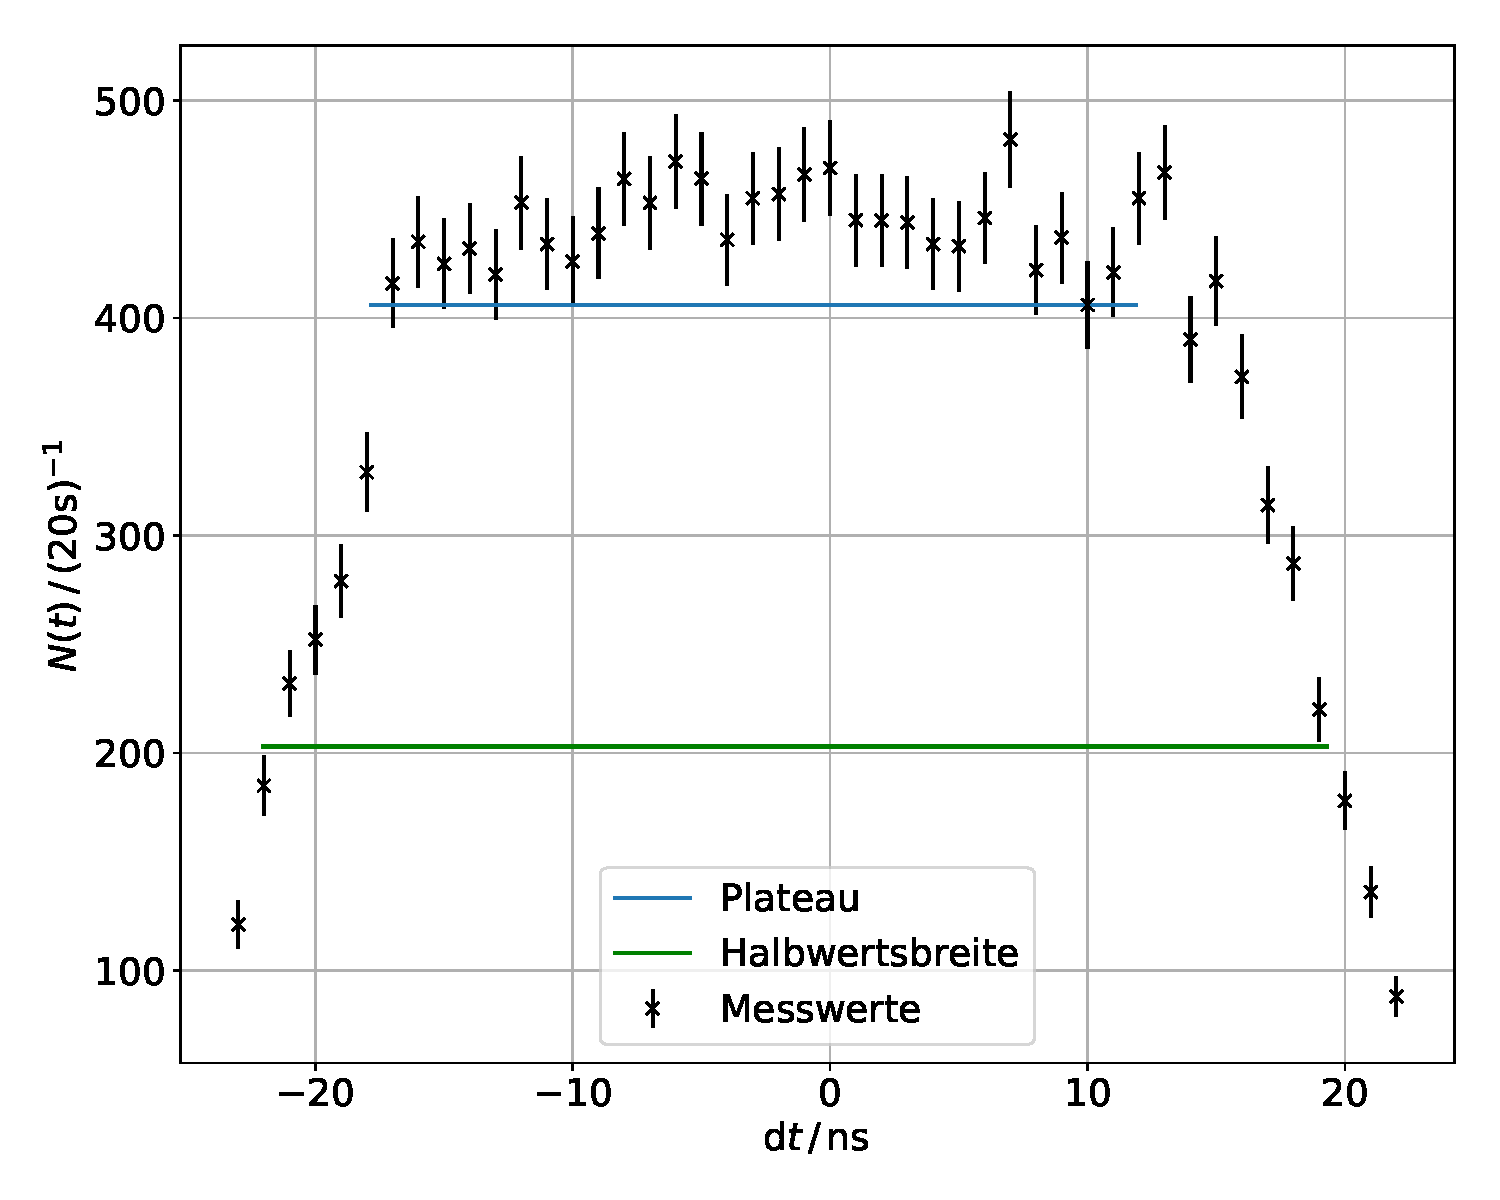
\includegraphics[width=0.59\textwidth]{Plateau20.pdf}
  \caption{Die graphische Darstellung der Messwerte.}
  \label{fig:2}
\end{figure}
\noindent
Für den Bereich von d$t$ = -17 bis d$t$ = 15 wird eine Konstante als Plateau gemittelt.
Für die Flanken wird mittels linearer Regression
\begin{equation*}
  f(x) = mx + b
\end{equation*}
je eine Gerade bestimmt.
Bei der Geraden rund um -20 auf der $dt/ns$-Achse ergibt sich:
\begin{align}
  m &= \SI{44(4)}{} \\
  b &= \SI{1.124(28)e3}{} \, .
\end{align}
Und bei der Geraden um 20 auf der $dt/ns$-Achse:
\begin{align}
  m &= \SI{-47.1(15)}{} \\
  b &= \SI{1.13(8)e3}{} \, .
\end{align}
In Abbildung \ref{fig:2} sind zusätzlich zu den Daten die Halbwertsbreite, das
Plateau und die linearen Näherungen der Flanken eingetragen.
Für die Auflösungszeit
$\symup{\Delta}t_K$ der Koinzidenzeinheit folgt durch Ablesen:
\begin{equation}
  \symup{\Delta}t_K = 2 \cdot \SI{20(1)}{\nano\second} - \SI{35(1)} = \SI{5(1)}{\nano\second} \, .
\end{equation}
Die Breite der Diskriminatoren ist etwa \SI{20}{\nano\second}. Die Halbwertsbreite sollte
etwa der doppelten Signalbreite der Diskriminatoren entsprechen, was ziemlich genau
erfüllt ist. Da die Schnittpunkte mit den Flanken je um \SI{-1}{\nano\second} verschoben
sind kann von einer entsprechenden optimalen Verzögerung ausgegangen werden.

\subsection{Kalibrierung der Kanäle}
\label{sec:kal}
Um die Kanäle zu kalibrieren, wird ein Doppelimpuls mit verschieden langen Impulsabständen
durch den Messaufbau geschickt und vom Vielkanalanalysator verarbeitet. Aus eben jenen
Impulsabständen $t_{\symup{kal}}$ und der Auswertung des Vielkanalanalysators lässt sich bestimmen, welcher
Kanal mit welchem Impulsabstand korrespondiert. Da sich diese proportional zueinander
verhalten, wird eine lineare Regression mit den Messwerten in Tabelle \ref{tab:2}
durchgeführt. Dabei wurden von den doppelt gefüllten Kanälen das gewichtete
arithmetische Mittel gebildet. Die Anzahl der Hits ist in Abbildung \ref{tab:2}
dargestellt.
Die lineare Regression
\begin{equation*}
  f(x) = mx + b
\end{equation*}
ist in Abbildung \ref{fig:3} zu sehen.

\begin{table}[H]
\centering
\begin{tabular}{c c c}
  \toprule
  $t_{\symup{kal}}$ / \si{\micro\second} & Kanal & \# Ereignisse \\
  \midrule
  1 & 22 & 1552 \\
  2 & 44 & 1328 \\
  3 & 66 & 1761 \\
  4 & 88 & 1015 \\
  5 & 110 & 1369 \\
  6 & 132 & 1266 \\
  7 & 154 & 1017 \\
  8 & 176 & 1549 \\
  9 & 198 & 2623 \\
  \bottomrule
\end{tabular}
  \caption{Die Anzahl der Hits auf den einzelnen Kanälen.}
  \label{tab:2}
\end{table}


\begin{figure}
  \centering
  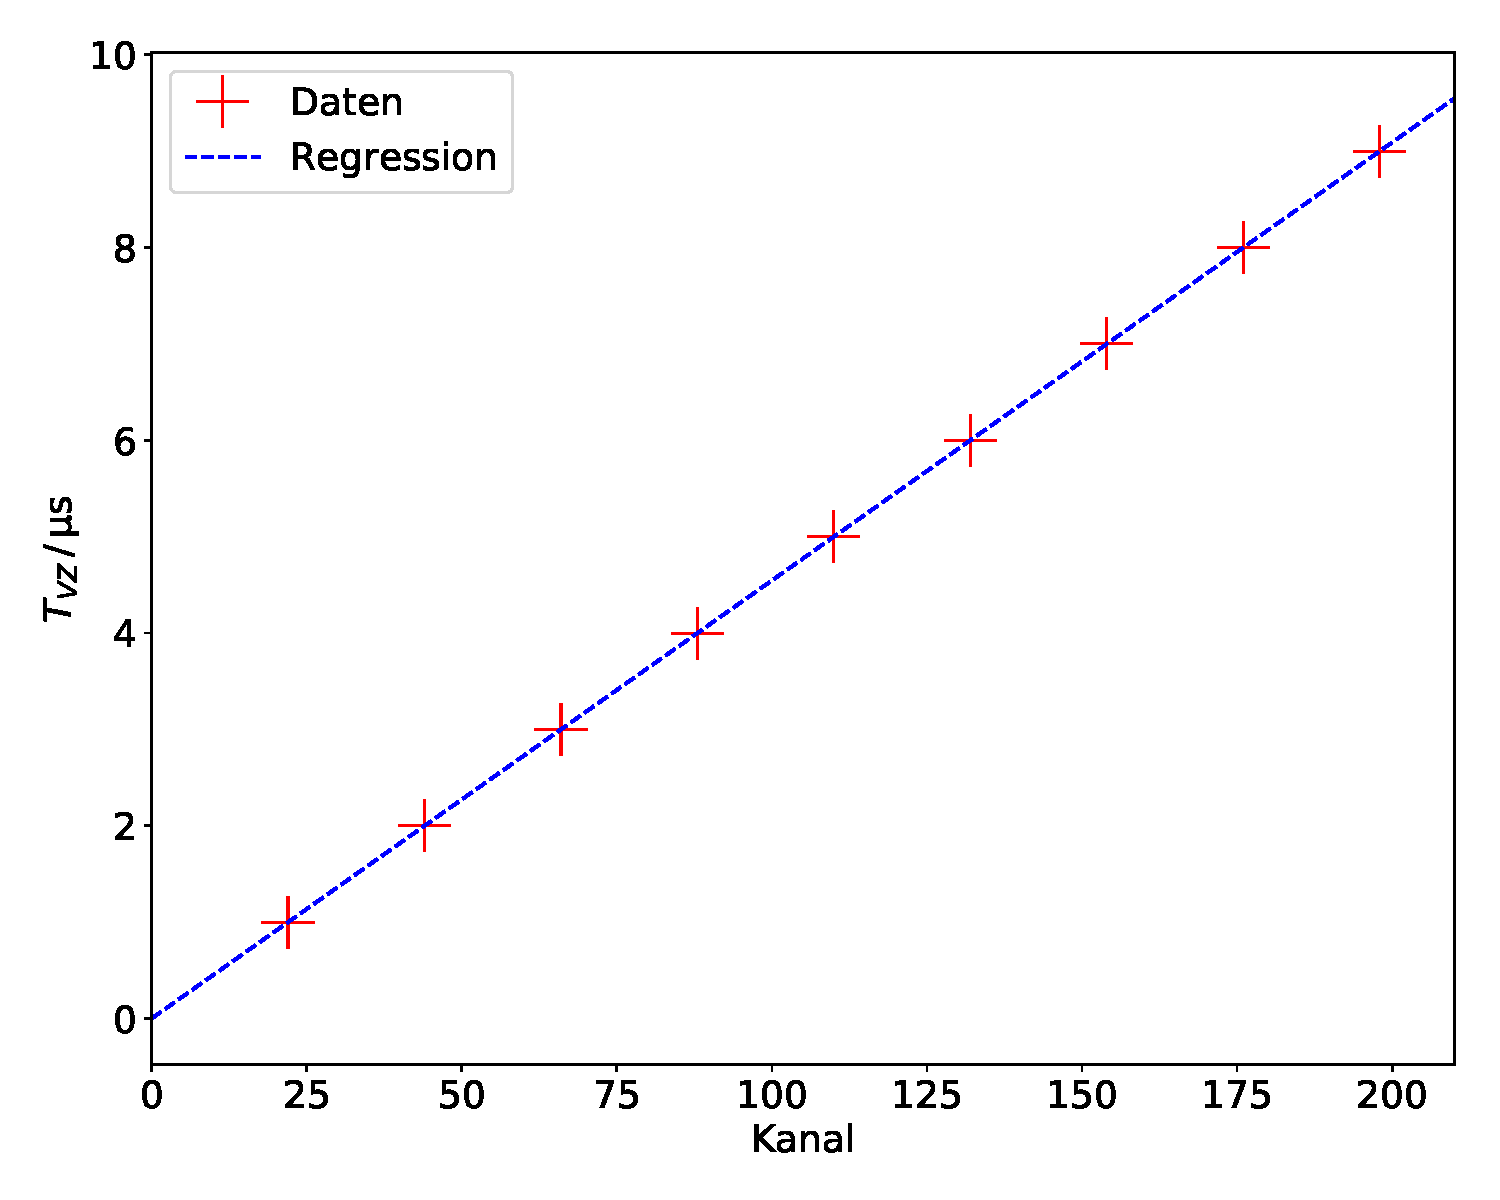
\includegraphics[width=0.59\textwidth]{kal20.pdf}
  \caption{Die grafische Darstellung der Messwerte für die Kalibrierung.}
  \label{fig:3}
\end{figure}
\noindent
Aus der linearen Regression folgen die Parameter:
\begin{align}
  m &= \num{0.04545(0000000003)} \\ ,
  b &= \SI{-2.1(000004)e-12}{\micro\second} \, .
\end{align}
Also lassen sich die zu den einzelnen
Kanälen gehörenden Zeitdauern aus einer linearen Funktion mit den errechneten
Parametern bestimmen. Dazu wurde angenommen, dass sich auch die Kanäle > 200
linear mit den errechneten Parametern verhalten.
\subsection{Bestimmung des Untergrundes}
Zunächst sich aus der Anzahl der Startimpulse und der gesamten Messzeit zu
\begin{equation}
  \overline{N} = \frac{N_{\symup{start}}}{T_{\symup{gesamt}}} \, .
\end{equation}
Während der Suchzeit $T_S$ tun dies im Mittel $n = \overline{N} \cdot T_S$ Myonen.
Die Wahrscheinlichkeit, dass dies genau $n$ Teilchen während der Suchzeit $T_S$
tun, ist poissonverteilt. Möchte man die Fehlmessungen $N_{\symup{fehl}}$
erhalten, so muss man genau die Fälle einbeziehen, in denen während der Suchzeit
zwei Myonen direkt aufeinander gefolgt sind, also die Anzahl aller Startimpulse
mit der zugehörigen Wahrscheinlichkeit, die man aus der Poissonverteilung
erhält, multiplizieren.
Mit $N_{\symup{start}} = \num{3.3937(18)e6}$, $T_S = \SI{20}{\micro\second}$ und $T_{\symup{gesamt}}
= \SI{153426}{\second}$ folgt
\begin{equation}
  N_{\symup{fehl}} = \overline{N} \cdot T_S \cdot \symup e^{- \overline{N} \cdot T_S}
  \cdot N_{\symup{start}} = \num{1500.7(16)} \, .
\end{equation}
Der Fehler von $N_{\symup{start}}$ bestimmt sich dabei ebenfalls als Poisson-Unsicherheit.
Da diese Ereignisse statistisch unabhängig voneinander sind, lässt sich die Untergrundrate
bestimmen aus
\begin{equation}
  U = \frac{N_{\symup{fehl}}}{\text{Anzahl Kanäle}} = \num{3.450(4)} \, .
\end{equation}
Dabei werden 435 Kanäle betrachtet, weil alle darüber hinaus leer sind bzw. lediglich
einer von ihnen ein Ereignis gemessen hat.

\subsection{Bestimmung der Lebensdauer}
Um die Lebensdauer zu bestimmen, werden als erstes die benutzten Kanäle in
Zeitdauern mit der linearen Regression aus Kapitel \ref{sec:kal} umgerechnet.
Die gemessenen Ereignisse werden dann in Abhängigkeit der bestimmten Zeitdauern
durch eine Funktion der Gestalt
\begin{equation}
  f(t) = N_0 \cdot \symup e^{-\lambda \, t} + U_{\symup{fit}} \, ,
  \label{fit}
\end{equation}
welche im Wesentlichen Gleichung \eqref{eq:expozerfall} plus der Untergrundrate entspricht,
mit \textsc{curve-fit} gefittet. Dabei wurde $(N)^{-1/2}$ als Gewichtung
genutzt, sodass die Werte mit viel Statistik (durch einen aussagekräftigeren, weil
mit mehr Werten unterlegten Fehler) stärker gewichtet werden als Werte mit niedrigem
$N(t)$. Es wurden insgesamt 41 der 512 Werte aus der Regression rausgenommen,
da diese keine Informationen enthielten, da sie außerhalb der Suchzeit aufgenommen wurden.
Die Messwerte und die Regression mit \eqref{fit} sind in
Abbildung \ref{fig:16} zu sehen.

\begin{figure}
  \centering
  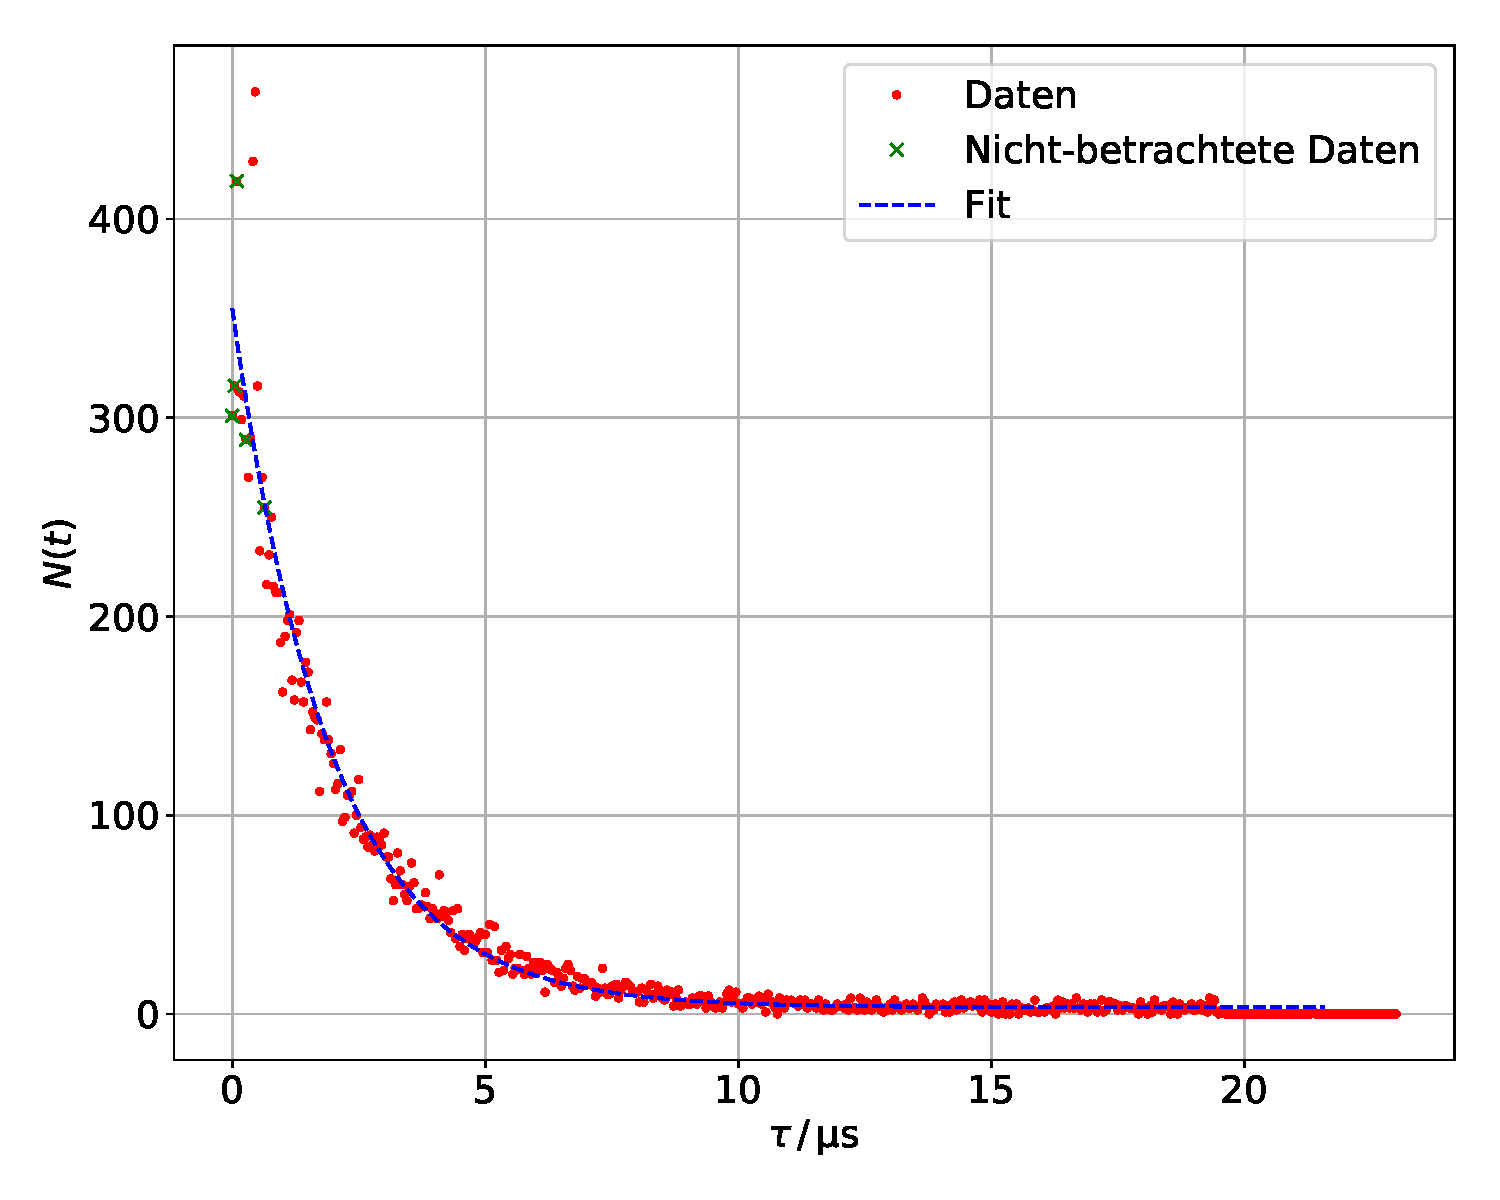
\includegraphics[scale=0.5]{fig24.pdf}
  \caption{Der Fit aller registrierten Myonen.}
  \label{fig:16}
\end{figure}
\noindent
Es ergeben sich für die Parameter:
\begin{align}
  N_0 &= \num{389(11)}, \\
  \lambda &= \SI{0.494(22)}{\per\micro\second} \label{dauer}, \\
  U_{\symup{fit}} &= \num{3.6(20)} \ \text{pro Kanal} \label{Untergrund} \, .
\end{align}
Aus \eqref{eq:tau} ergibt sich für die Lebensdauer
\begin{equation}
  \tau = \SI{2.08(9)}{\micro\second} \, .
\end{equation}
\clearpage
\section{Diskussion}
\begin{table}
  \centering
  \caption{Errechnete und gefittete Werte für die Lebensdauer und die Untergrundrate.}
  \label{tab:dis}
  \begin{tabular}{c c c}
    \toprule
     &Wert aus Fit & Wert aus Literatur / Berechnung \\
    \midrule
    $\tau$ & \SI{2.02(9)}{\micro\second} & \SI{2.197}{\micro\second} \cite{literaturwert} \\
    $U$ & \num{2.5(20)} \ \text{pro Kanal} & \num{3.450(4)} \ \text{pro Kanal} \\
    \bottomrule
  \end{tabular}
\end{table}
\noindent
Es wird ersichtlich, dass die Untergrundraten stark voneinander
abweichen, aber der aus dem Fit bestimmte Wert auch eine sehr große Abweichung hat.
Dies liegt an den statistischen Schwankungen bei den hohen Lebensdauern. Insgesamt
passen die Werte unter Berücksichtigung der Fehlerbereiche, zusammen. \\
\\
Der Literaturwert für die Lebensdauer liegt leicht oberhalb der errechneten Lebensdauer.
Grund dafür sind wahrscheinlich die größeren Ausreißer im unteren Zeitbereich.
Zu den nicht-betrachteten Werten lässt sich sagen, dass nur der Wert an der Stelle
(0,0) rausgelassen wurde, da dieser schlichtweg physikalisch nicht sinnvoll ist.
Insgesamt lässt sich vermuten, dass vorallem die hohe Anzahl an Ereignissen
für gute statistische Werte und verhältnismäßig kleine Unsicherheiten sorgt. Insgesamt
lässt sich als Fehlerquelle vermuten, dass die Einstellung der Schwelle der Diskriminatoren
sowie die optimale Verzögerung in der Koinzidenzschaltung ungenau sind, da diese mit
einer Stoppuhr und von Hand vermessen wurden.
Die Auflösungszeit $\symup \Delta t_K$ liegt bei \SI{5}{\nano\second}.\\
\\
Die Summe aller Ereignisse aus dem Vielkanalanalysator beträgt \num{1.84(20)e4} mit
einem Poissonfehler, die
am Zählwerk \num{17818}. Die Anzahl am Zählwerk liegt sehr gut in der Fehlertoleranz der
Summe aus dem Vielkanalanalysator.

\newpage
\nocite{*}
\printbibliography
\end{document}
